\section{Sampling Distributions}

This section groups the technical tools that underpin sampling distributions. The distributions studied here (Z, t, $\chi^2$, F) are the backbone of classical statistical inference and appear recurrently in data science problems.


\subsection{Transformation of Random Variables}

A frequent question in statistics is: if $X$ has a known distribution and we define $Y = g(X)$ for some function $g$, what is the distribution of $Y$?

\subsubsection{Linear Transformation}

\begin{teorema}[Affine Transformation]
If $X$ is a random variable with mean $\mu_X$ and variance $\sigma_X^2$, and $Y = aX + b$ with $a \neq 0$, then
\begin{align}
 \label{eq:3.2.1}
 \mu_Y &= a\mu_X + b, \\
 \label{eq:3.2.2}
 \sigma_Y^2 &= a^2\sigma_X^2.
\end{align}
Furthermore, if $X$ has cumulative distribution function $F_X$, then
$F_Y(y) = F_X\!\left(\frac{y-b}{a}\right)$.
\end{teorema}

\begin{ejemplo}
 \label{exmp:3.2.1}
If $X \sim N(\mu, \sigma^2)$ and $Y = aX + b$ with $a \neq 0$, then
$Y \sim N(a\mu + b, a^2\sigma^2)$. This is the \emph{reproductive property} of the normal distribution under linear transformations.
\end{ejemplo}

\subsubsection{Change of Variable Theorem}

For more general transformations, we need the following result.

\begin{teorema}[Change of Variable, Monotone Case]
Let $X$ be a continuous random variable with density $f_X$, and $g$ a strictly monotone and differentiable function. If $Y = g(X)$ and $g^{-1}$ denotes the inverse of $g$, then the density of $Y$ is
\begin{align}
 \label{eq:3.2.3}
 f_Y(y) = f_X\!\left(g^{-1}(y)\right) \cdot \left|\frac{d}{dy}\,g^{-1}(y)\right|,
\end{align}
for all $y$ in the range of $g$.
\end{teorema}

\begin{proof}
Suppose $g$ is increasing. For $y$ in the range of $g$,
\begin{align}
 F_Y(y) = P(Y \leq y) = P(g(X) \leq y) = P(X \leq g^{-1}(y)) = F_X(g^{-1}(y)).
\end{align}
Differentiating and applying the chain rule,
\begin{align}
 f_Y(y) = \frac{d}{dy} F_X(g^{-1}(y)) = f_X(g^{-1}(y)) \cdot \frac{d}{dy} g^{-1}(y).
\end{align}
The decreasing case is analogous, taking the absolute value.
\end{proof}

\begin{observacion}[Alternative Form]
If we write $x = g^{-1}(y)$ and denote $J(y) = \frac{dx}{dy}$ the Jacobian of the inverse transformation, the formula can be rewritten as
\begin{align}
 \label{eq:3.2.4}
 f_Y(y) = f_X(x)\,|J(y)|, \quad \text{where } x = g^{-1}(y).
\end{align}
In higher dimensions, $|J(y)|$ is the absolute value of the Jacobian determinant.
\end{observacion}

\begin{ejemplo}
 \label{exmp:3.2.2}
Let $X \sim \text{Exp}(1)$ with density $f_X(x) = e^{-x}$ for $x > 0$. Find the distribution of $Y = e^X$.
\end{ejemplo}

\begin{solucion}
The transformation $g(x) = e^x$ is strictly increasing from $(0, \infty)$ to $(1, \infty)$, with inverse $g^{-1}(y) = \ln y$. Furthermore, $\frac{d}{dy}\ln y = 1/y$.

By the change of variable theorem, for $y > 1$:
\begin{align}
 f_Y(y) = f_X(\ln y) \cdot \frac{1}{y} = e^{-\ln y} \cdot \frac{1}{y} = \frac{1}{y} \cdot \frac{1}{y} = \frac{1}{y^2}.
\end{align}

Therefore, $Y$ has density $f_Y(y) = 1/y^2$ for $y > 1$ (a Pareto distribution with parameter $\alpha = 1$).
\end{solucion}

\begin{ejemplo}
 \label{exmp:3.2.3}
Let $X \sim N(\mu, \sigma^2)$. Find the distribution of $Y = e^X$ (the \emph{log-normal} distribution).
\end{ejemplo}

\begin{solucion}
The transformation $g(x) = e^x$ is increasing, with inverse $g^{-1}(y) = \ln y$. The density of $X$ is
\begin{align}
 f_X(x) = \frac{1}{\sigma\sqrt{2\pi}}\,\exp\!\left(-\frac{(x-\mu)^2}{2\sigma^2}\right).
\end{align}

Applying the theorem, for $y > 0$:
\begin{align}
 f_Y(y) &= f_X(\ln y) \cdot \frac{1}{y} \\
 &= \frac{1}{\sigma\sqrt{2\pi}}\,\exp\!\left(-\frac{(\ln y - \mu)^2}{2\sigma^2}\right) \cdot \frac{1}{y}.
\end{align}

Therefore, $Y$ follows a log-normal distribution $LN(\mu, \sigma^2)$.
\end{solucion}

\begin{ejemplo}
 \label{exmp:3.2.4}
Let $X \sim U(0, 2\pi)$ be uniformly distributed. Find the distribution of $Y = \sin(X)$ (non-monotone case).
\end{ejemplo}

\begin{solucion}
The function $g(x) = \sin x$ is not monotone on $(0, 2\pi)$: it reaches a maximum of $1$ at $x = \pi/2$ and a minimum of $-1$ at $x = 3\pi/2$. Each value $y \in (-1, 1)$ has two preimages: $x_1 = \arcsin y$ and $x_2 = \pi - \arcsin y$.

Using the formula for the non-monotone case,
\begin{align}
 f_Y(y) &= \sum_{x: \sin x = y} f_X(x) \cdot \left|\frac{dx}{dy}\right| \\
 &= \frac{1}{2\pi}\cdot\frac{1}{\sqrt{1-y^2}} + \frac{1}{2\pi}\cdot\frac{1}{\sqrt{1-y^2}} \\
 &= \frac{1}{\pi\sqrt{1-y^2}}, \quad y \in (-1, 1).
\end{align}

This is the density of the \emph{arcsine distribution}, which appears in the \emph{random walk}.
\end{solucion}

\subsubsection{Common Transformations}

\begin{observacion}
The following transformations are useful for \emph{normalizing} data or stabilizing variances:
\begin{itemize}
 \item $Y = \ln X$: compresses large values, expands values close to $0$.
 \item $Y = \sqrt{X}$: smooths out the skewness of count data.
 \item $Y = X^{1/3}$: alternative to the square root for data with pronounced skewness.
 \item \emph{Box-Cox}: $Y = (X^\lambda - 1)/\lambda$ for $\lambda \neq 0$; $Y = \ln X$ for $\lambda = 0$. Optimizes normality.
\end{itemize}
\end{observacion}

\lstinputlisting[language=Python]{../code/distribuciones-muestreo/transformacionesVariables.py}

\begin{figure}
 \centering
 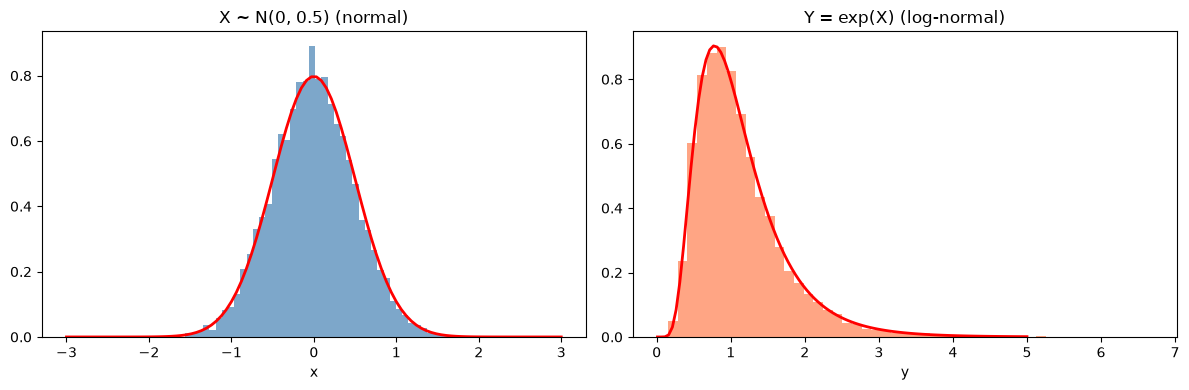
\includegraphics[height=7cm,keepaspectratio=true]{./pe/transformaciones.png}
 % transformaciones.png: 0x0 pixel, 300dpi, 0.00x0.00 cm, bb=
 \caption{Exponential transformation: from normal to log-normal.}
 \label{fig:3.2.1}
\end{figure}



\subsection{Distributions of Functions of Random Variables}

This subsection generalizes the previous results to the case where $Y$ is a function (not necessarily monotone) of $X$ or of several variables.

\subsubsection{Single Variable Case}

When $g$ is not monotone, we must consider all preimages of each value $y$. The general formula is
\begin{align}
 \label{eq:3.2.5}
 f_Y(y) = \sum_{x \in g^{-1}(y)} f_X(x) \cdot \left|\frac{dx}{dy}\right|
 = \sum_{x: g(x) = y} \frac{f_X(x)}{|g'(x)|}.
\end{align}

\begin{observacion}
The condition $|g'(x)| \neq 0$ at each $x \in g^{-1}(y)$ guarantees that the transformation is locally invertible at each preimage.
\end{observacion}

\subsubsection{Multivariate Case}

If $(X_1, \ldots, X_n)$ has joint density $f_{X_1, \ldots, X_n}$ and $Y = g(X_1, \ldots, X_n)$, the density of $Y$ is obtained by integrating the joint density over the level set $g(x_1, \ldots, x_n) = y$:
\begin{align}
 \label{eq:3.2.6}
 f_Y(y) = \int \cdots \int_{g(x_1, \ldots, x_n) = y} f_{X_1, \ldots, X_n}(x_1, \ldots, x_n)
 	\cdot \frac{dS}{|\nabla g|},
\end{align}
where $dS$ is the surface area element on the level set and $\nabla g$ is the gradient of $g$.

\begin{ejemplo}
 \label{exmp:3.2.5}
If $X_1, X_2 \sim \text{Exp}(1)$ are independent, find the distribution of $Y = X_1 + X_2$.
\end{ejemplo}

\begin{solucion}
The joint probability density function is $f(x_1, x_2) = e^{-(x_1+x_2)}$ for $x_1, x_2 > 0$. The sum $Y = X_1 + X_2$ is obtained by integrating along the line $x_1 + x_2 = y$:
\begin{align}
 f_Y(y) &= \int_0^y e^{-(x_1 + (y-x_1))}\,dx_1 = \int_0^y e^{-y}\,dx_1 = y\,e^{-y}, \quad y > 0.
\end{align}

This is the Erlang density with shape parameter $2$, or equivalently $\text{Gamma}(2, 1)$. Generalizing, the sum of $n$ iid exponential random variables is $\text{Gamma}(n, 1)$ (see Section 2.11).
\end{solucion}



\subsection{Sampling Distributions of Means}

The sampling distribution of the mean is fundamental for statistical inference. Its detailed treatment is carried out in Section \ref{sec:3.4}; here we summarize the main results.

If $X_1, X_2, \ldots, X_n$ are independent and identically distributed (iid) random variables with mean $\mu$ and variance $\sigma^2$, and $\bar{X} = \frac{1}{n}\sum X_i$, then
\begin{align}
 \label{eq:3.2.7}
 E(\bar{X}) &= \mu, \\
 \label{eq:3.2.8}
 \text{Var}(\bar{X}) &= \frac{\sigma^2}{n}, \\
 \label{eq:3.2.9}
 \text{SD}(\bar{X}) &= \frac{\sigma}{\sqrt{n}}.
\end{align}

Furthermore, by the Central Limit Theorem, when $n$ is sufficiently large,
\begin{align}
 \label{eq:3.2.10}
 \frac{\bar{X} - \mu}{\sigma/\sqrt{n}} \xrightarrow{d} N(0,1).
\end{align}

\begin{observacion}
The exact distribution of $\bar{X}$ is \emph{normal} if the original population is normal, and approximately normal for large $n$ in other cases. This difference is crucial: in the first case we speak of an exact $Z$; in the second, of an approximate $Z$.
\end{observacion}



\subsection{Statistics and the Unbiased Sample Variance}

\begin{definicion}[Statistic]
Let $X_1, X_2, \ldots, X_n$ be a simple random sample (iid random variables) from a population. A \emph{statistic} is any function $T = g(X_1, \ldots, X_n)$ of the sample that does not depend on unknown population parameters. Every statistic is itself a random variable with its own probability distribution, called the \emph{sampling distribution} of $T$.
\end{definicion}

The sample mean $\bar{X}$ is the most commonly used statistic; the second most important is the \emph{sample variance}.

\begin{definicion}[Sample variance]
 \label{eq:5.1.1}
Given a simple random sample $X_1, \ldots, X_n$ with sample mean $\bar{X}$, the \emph{sample variance} is defined as
\begin{align}
 S^2 = \frac{1}{n-1}\sum_{i=1}^n (X_i - \bar{X})^2.
\end{align}
\end{definicion}

\begin{observacion}[Why divide by $n-1$ instead of $n$?]
The divisor $n-1$ (known as \emph{Bessel's correction}) is not arbitrary: it is precisely what makes $S^2$ an \emph{unbiased estimator} of the population variance $\sigma^2$, as shown below.
\end{observacion}

\begin{teorema}[Unbiasedness of the sample variance]
 \label{eq:5.1.2}
If $X_1, \ldots, X_n$ are iid with mean $\mu$ and variance $\sigma^2 < \infty$, then
\begin{align}
 E(S^2) = \sigma^2.
\end{align}
\end{teorema}

\begin{proof}
We write the sum of squares centered at $\bar{X}$ in terms of the population mean $\mu$, adding and subtracting $\mu$:
\begin{align}
 \sum_{i=1}^n (X_i - \bar{X})^2
 &= \sum_{i=1}^n \left[(X_i - \mu) - (\bar{X} - \mu)\right]^2 \\
 &= \sum_{i=1}^n (X_i - \mu)^2 - 2(\bar{X}-\mu)\sum_{i=1}^n(X_i-\mu) + n(\bar{X}-\mu)^2 \\
 &= \sum_{i=1}^n (X_i - \mu)^2 - n(\bar{X}-\mu)^2,
\end{align}
where we used $\sum_{i=1}^n (X_i - \mu) = n(\bar{X}-\mu)$. Taking expectations and using $E[(X_i-\mu)^2] = \sigma^2$ for each $i$, and $E[(\bar{X}-\mu)^2] = \text{Var}(\bar{X}) = \sigma^2/n$:
\begin{align}
 E\left[\sum_{i=1}^n (X_i - \bar{X})^2\right] = n\sigma^2 - n\cdot\frac{\sigma^2}{n}
 = (n-1)\sigma^2.
\end{align}
Dividing by $n-1$:
\begin{align}
 E(S^2) = E\left[\frac{1}{n-1}\sum_{i=1}^n (X_i - \bar{X})^2\right]
 = \frac{(n-1)\sigma^2}{n-1} = \sigma^2. \qedhere
\end{align}
\end{proof}

\begin{observacion}[The ``natural'' estimator is biased]
The estimator that divides by $n$ instead of $n-1$, $\hat{\sigma}^2 = \frac{1}{n}\sum(X_i-\bar{X})^2 = \frac{n-1}{n}S^2$, systematically \emph{underestimates} the population variance:
\begin{align}
 E(\hat{\sigma}^2) = \frac{n-1}{n}\sigma^2 < \sigma^2.
\end{align}
Intuitively, $\bar{X}$ is, by construction, closer to each $X_i$ than the unknown population mean $\mu$, so the sum of squares around $\bar{X}$ underestimates the true spread; dividing by $n-1$ instead of $n$ (``losing one degree of freedom'' from having estimated $\mu$ with $\bar{X}$) corrects exactly for that bias.
\end{observacion}

\begin{ejemplo}
 \label{exmp:5.1.1}
A simple random sample of size $n=5$ yields the observations $\{12, 15, 11, 18, 14\}$. Compute the sample mean $\bar{X}$ and the unbiased sample variance $S^2$.
\end{ejemplo}

\begin{solucion}
The sample mean is
\begin{align}
 \bar{X} = \frac{12+15+11+18+14}{5} = \frac{70}{5} = 14.
\end{align}
The squared deviations are $(12-14)^2=4$, $(15-14)^2=1$, $(11-14)^2=9$, $(18-14)^2=16$, $(14-14)^2=0$, summing to $30$. Therefore,
\begin{align}
 S^2 = \frac{1}{n-1}\sum_{i=1}^n (X_i-\bar{X})^2 = \frac{30}{4} = 7.5.
\end{align}
\end{solucion}



\subsection{Central Limit Theorem: Asymptotic Convergence}

\begin{definicion}[Convergence in distribution]
A sequence of random variables $Y_n$ \emph{converges in distribution} to $Y$ (written $Y_n \xrightarrow{d} Y$) if $F_{Y_n}(y) \to F_Y(y)$ at every continuity point of $F_Y$.
\end{definicion}

\begin{teorema}[Central Limit Theorem (Lindeberg--L\'evy)]
 \label{eq:5.2.1}
Let $X_1, X_2, \ldots$ be iid random variables with mean $\mu$ and variance $\sigma^2 < \infty$. Then
\begin{align}
 Z_n = \frac{\bar{X}_n - \mu}{\sigma/\sqrt{n}} \xrightarrow{d} N(0,1)
 \quad \text{as } n \to \infty.
\end{align}
\end{teorema}

\begin{proof}[Proof sketch via MGF]
Suppose $M_{X_1}(t)$ exists in a neighborhood of $t=0$. The MGF of $Z_n$ is
\begin{align}
 M_{Z_n}(t) = e^{-\mu t \sqrt{n}/\sigma}\left[M_{X_1}\!\left(\frac{t}{\sigma\sqrt{n}}\right)\right]^n.
\end{align}
Expanding $\log M_{X_1}(s)$ in a Taylor series around $s=0$:
\begin{align}
 \log M_{X_1}(s) = \mu s + \frac{\sigma^2 s^2}{2} + O(s^3).
\end{align}
Substituting $s = t/(\sigma\sqrt{n})$ and multiplying by $n$:
\begin{align}
 \log M_{Z_n}(t) = n\left[\frac{\mu t}{\sigma\sqrt{n}} + \frac{t^2}{2n} + O(n^{-3/2})\right]
 - \frac{\mu t\sqrt{n}}{\sigma} = \frac{t^2}{2} + O(n^{-1/2}) \;\longrightarrow\; \frac{t^2}{2}.
\end{align}
Hence $M_{Z_n}(t) \to e^{t^2/2}$, the MGF of $N(0,1)$; by L\'evy's uniqueness and continuity theorem, $Z_n \xrightarrow{d} N(0,1)$.
\end{proof}

\begin{observacion}[Independence from the original distribution]
The result does not depend on the shape of the distribution of $X_i$ (discrete, continuous, symmetric, skewed) --- it only requires finite mean and variance. This universality is why the CLT is the cornerstone of classical statistical inference.
\end{observacion}

\subsubsection{Rate of convergence: the Berry--Esseen theorem}

The CLT guarantees convergence as $n \to \infty$, but says nothing about how fast. The following result quantifies the error of the normal approximation for finite $n$.

\begin{teorema}[Berry--Esseen]
 \label{eq:5.2.2}
Let $X_1,\ldots,X_n$ be iid with $E|X_i-\mu|^3 = \rho < \infty$. There exists a universal constant $C$ (known to satisfy $C < 0.5$) such that
\begin{align}
 \sup_z \left|F_{Z_n}(z) - \Phi(z)\right| \le \frac{C\rho}{\sigma^3\sqrt{n}}.
\end{align}
\end{teorema}

\begin{observacion}[The practical rule $n \ge 30$]
The Berry--Esseen theorem confirms that the error of the normal approximation decays as $O(1/\sqrt{n})$: quadrupling $n$ halves the maximum error. The popular ``$n \ge 30$'' rule is a reasonable heuristic for moderately symmetric populations with finite moments, but heavily skewed or heavy-tailed distributions (i.e., with large $\rho$) require larger $n$ to reach the same precision.
\end{observacion}

\begin{ejemplo}
 \label{exmp:5.2.1}
Service time at a call center follows an exponential distribution with mean $\mu = 1/\lambda = 4$ minutes and standard deviation $\sigma = 4$. A sample of $n=64$ calls is taken. What is the approximate probability that the average service time exceeds $4.5$ minutes?
\end{ejemplo}

\begin{solucion}
By the CLT, $\bar{X}_{64} \approx N(4, \sigma^2/n) = N(4, 16/64) = N(4, 0.25)$, with standard deviation $\text{SD}(\bar{X}) = 0.5$.
\begin{align}
 P(\bar{X} > 4.5) \approx P\!\left(Z > \frac{4.5-4}{0.5}\right) = P(Z>1) = 1-\Phi(1)
 \approx 0.1587.
\end{align}
\end{solucion}



\subsection{Chi-Square ($\chi^2$) Distribution}

The $\chi^2$ distribution arises when summing squares of standard normal random variables. Its detailed treatment is carried out in Section \ref{sec:3.9}; here we present the essential results.

\begin{definicion}[$\chi^2$ Distribution]
Let $Z_1, Z_2, \ldots, Z_\nu$ be independent random variables with $Z_i \sim N(0,1)$. The random variable
\begin{align}
 \label{eq:3.2.11}
 \chi^2_\nu = \sum_{i=1}^\nu Z_i^2
\end{align}
follows a \emph{chi-square} distribution with $\nu$ degrees of freedom.
\end{definicion}

{Properties}
\begin{itemize}
 \item Mean: $E(\chi^2_\nu) = \nu$.
 \item Variance: $\text{Var}(\chi^2_\nu) = 2\nu$.
 \item As a special case of the gamma family (Section 2.11), $\chi^2_\nu = \text{Gamma}\!\left(\frac{\nu}{2}, 2\right)$.
 \item Reproductive property: if $\chi^2_{\nu_1}$ and $\chi^2_{\nu_2}$ are independent, $\chi^2_{\nu_1} + \chi^2_{\nu_2} \sim \chi^2_{\nu_1 + \nu_2}$.
\end{itemize}

\begin{observacion}
The $\chi^2$ distribution arises naturally when estimating the variance of a normal population. If $X_1, \ldots, X_n$ are iid normal and $S^2$ is the sample variance, then
\begin{align}
 \frac{(n-1)S^2}{\sigma^2} \sim \chi^2_{n-1}.
\end{align}
This result forms the basis for confidence intervals for $\sigma^2$ and for the chi-square goodness-of-fit test.
\end{observacion}

\begin{definicion}[Chi-square density]
 \label{eq:5.3.1}
As a special case of the gamma distribution with $\alpha=\nu/2$ and $\beta=2$, the density function of $\chi^2_\nu$ is
\begin{align}
 f(x) = \frac{1}{2^{\nu/2}\Gamma(\nu/2)}\,x^{\nu/2-1}e^{-x/2}, \qquad x > 0.
\end{align}
\end{definicion}

\begin{teorema}[Fisher's Theorem]
 \label{eq:5.3.2}
Let $X_1, \ldots, X_n$ be iid random variables with $X_i \sim N(\mu, \sigma^2)$, with sample mean $\bar{X}$ and sample variance $S^2$. Then:
\begin{enumerate}
 \item $\bar{X}$ and $S^2$ are \emph{independent};
 \item $\dfrac{(n-1)S^2}{\sigma^2} \sim \chi^2_{n-1}$.
\end{enumerate}
\end{teorema}

\begin{observacion}[Idea of the proof]
The independence of $\bar{X}$ and $S^2$ is a surprising result: even though $S^2$ is computed from the deviations $(X_i-\bar{X})$, which depend on $\bar{X}$, the vector of deviations turns out to be statistically independent of $\bar{X}$ when the population is normal. The formal proof uses an orthogonal transformation of the vector $(X_1,\ldots,X_n)$ that separates the direction of $\bar{X}$ (a single degree of freedom) from the remaining $n-1$ orthogonal directions, each capturing information independent of $\bar X$; the sum of squares along those $n-1$ directions is exactly $(n-1)S^2$, which explains both the independence and the $n-1$ degrees of freedom (this is a special case of \emph{Cochran's theorem}).
\end{observacion}

\begin{ejemplo}
 \label{exmp:5.3.1}
The fill volume of soda cans from a bottling plant follows $N(\mu, \sigma^2=4)$ (in milliliters, with $\sigma=2$). A sample of $n=10$ cans is taken and $S^2 = 7.2$ is computed. What is the value of the statistic $(n-1)S^2/\sigma^2$, and how extreme is this value compared to the $\chi^2_9$ distribution (whose expected value is $9$)?
\end{ejemplo}

\begin{solucion}
The statistic is
\begin{align}
 \frac{(n-1)S^2}{\sigma^2} = \frac{9 \cdot 7.2}{4} = \frac{64.8}{4} = 16.2.
\end{align}
Since $16.2 > 9 = E(\chi^2_9)$, the observed sample variance is larger than expected under $\sigma^2=4$. Using $\chi^2_9$ tables, the $95\%$ critical value is $\chi^2_{9,0.95} \approx 16.92$; since $16.2 < 16.92$, the value is not extreme enough to reject $\sigma^2=4$ at the $\alpha=0.05$ level (though it is close to the threshold).
\end{solucion}



\subsection{Student's $t$-Distribution}

The $t$-distribution arises when we standardize a sample mean using the sample standard deviation (which is a random variable) instead of the population standard deviation.

\begin{definicion}[Student's $t$-Distribution]
Let $Z \sim N(0,1)$ and $\chi^2_\nu$ be a chi-square variable with $\nu$ degrees of freedom, independent of each other. Then
\begin{align}
 \label{eq:3.2.12}
 T = \frac{Z}{\sqrt{\chi^2_\nu / \nu}}
\end{align}
follows a \emph{Student's $t$-distribution} with $\nu$ degrees of freedom. We write $T \sim t_\nu$.
\end{definicion}

{Properties}
\begin{itemize}
 \item The probability density function of $T$ is
 \begin{align}
  \label{eq:3.2.13}
  f(t) = \frac{\Gamma\!\left(\frac{\nu+1}{2}\right)}{\sqrt{\nu\pi}\,\Gamma\!\left(\frac{\nu}{2}\right)}
  \left(1 + \frac{t^2}{\nu}\right)^{-(\nu+1)/2}, \quad t \in \mathbb{R}.
 \end{align}
 \item $E(T) = 0$ for $\nu > 1$.
 \item $\text{Var}(T) = \nu/(\nu - 2)$ for $\nu > 2$.
 \item As $\nu \to \infty$, $T \xrightarrow{d} N(0,1)$. For small $\nu$, $T$ has heavier tails than the normal distribution.
\end{itemize}

\begin{observacion}
The $t$-distribution arises when estimating the mean $\mu$ with unknown $\sigma$: if $X_1, \ldots, X_n \sim N(\mu, \sigma^2)$ iid and $S^2$ is the sample variance, then
\begin{align}
 \label{eq:3.2.14}
 \frac{\bar{X} - \mu}{S/\sqrt{n}} \sim t_{n-1}.
\end{align}
This is the \emph{$t$-statistic} that gives its name to the $t$-test (Section 3.6).
\end{observacion}



\subsection{Snedecor's $F$-Distribution}

The $F$-distribution is fundamental for comparing variances and in the Analysis of Variance (ANOVA).

\subsubsection{Definition}

\begin{definicion}[$F$-Distribution]
Let $\chi^2_{d_1}$ and $\chi^2_{d_2}$ be independent chi-square random variables with $d_1$ and $d_2$ degrees of freedom, respectively. The random variable
\begin{align}
 \label{eq:3.2.15}
 F = \frac{\chi^2_{d_1}/d_1}{\chi^2_{d_2}/d_2}
\end{align}
follows a \emph{Snedecor's $F$-distribution} with $(d_1, d_2)$ degrees of freedom. We write $F \sim F_{d_1, d_2}$.
\end{definicion}

{Properties}
\begin{itemize}
 \item $F \geq 0$ and the distribution is asymmetric (right-skewed).
 \item The probability density function of $F$ is
 \begin{align}
  \label{eq:3.2.16}
  f(x) = \frac{1}{B(d_1/2, d_2/2)} \left(\frac{d_1}{d_2}\right)^{d_1/2}
  x^{d_1/2 - 1} \left(1 + \frac{d_1}{d_2}x\right)^{-(d_1+d_2)/2},
  \end{align}
  where $B$ is the beta function.
 \item $E(F) = d_2/(d_2 - 2)$ for $d_2 > 2$.
 \item $\text{Var}(F) = \dfrac{2 d_2^2 (d_1 + d_2 - 2)}{d_1 (d_2 - 2)^2 (d_2 - 4)}$ for $d_2 > 4$.
 \item If $F \sim F_{d_1, d_2}$, then $1/F \sim F_{d_2, d_1}$.
\end{itemize}

\subsubsection{Application: Comparing Two Variances}

If $X_1, \ldots, X_{n_1} \sim N(\mu_1, \sigma_1^2)$ and $Y_1, \ldots, Y_{n_2} \sim N(\mu_2, \sigma_2^2)$ are independent samples, the ratio of sample variances
\begin{align}
 \label{eq:3.2.17}
 F = \frac{S_1^2}{S_2^2}
\end{align}
follows an $F_{n_1 - 1, n_2 - 1}$ distribution under the null hypothesis $H_0: \sigma_1^2 = \sigma_2^2$. This is the \emph{$F$-test for equality of variances}.

\subsubsection{Application: ANOVA}

The Analysis of Variance (ANOVA) decomposes the total variability of data into components attributable to different factors.

\begin{teorema}[$F$-Statistic in ANOVA]
Consider $k$ groups with $n_i$ observations in the $i$-th group, and denote
\begin{align}
 \text{SS}_{\text{treat}} &= \sum_{i=1}^k n_i (\bar{X}_i - \bar{X})^2, \\
 \text{SS}_{\text{error}} &= \sum_{i=1}^k \sum_{j=1}^{n_i} (X_{ij} - \bar{X}_i)^2.
\end{align}
If $H_0: \mu_1 = \cdots = \mu_k$ is true, then
\begin{align}
 \label{eq:3.2.18}
 F = \frac{\text{SS}_{\text{treat}}/(k-1)}{\text{SS}_{\text{error}}/(n-k)} \sim F_{k-1, n-k},
\end{align}
where $n = \sum n_i$.
\end{teorema}

\begin{ejemplo}
 \label{exmp:3.2.6}
We want to compare the average performance of three teaching methods. The three methods are applied to groups of $5$ students each, obtaining the following scores:
\begin{align}
 \text{Method A: } 85, 90, 78, 92, 88 \quad (\bar{X}_A = 86.6), \\
 \text{Method B: } 79, 81, 85, 77, 83 \quad (\bar{X}_B = 81.0), \\
 \text{Method C: } 92, 95, 88, 90, 93 \quad (\bar{X}_C = 91.6).
\end{align}
Is there evidence that the methods produce different results?
\end{ejemplo}

\begin{solucion}
We calculate the variance components:
\begin{align}
 \bar{X} &= \frac{86.6 + 81.0 + 91.6}{3} = 86.4, \\
 \text{SS}_{\text{treat}} &= 5(86.6 - 86.4)^2 + 5(81.0 - 86.4)^2 + 5(91.6 - 86.4)^2 = 290.0, \\
 \text{SS}_{\text{error}} &= \text{within-group variance} \times (n - k).
\end{align}
To simplify, let us denote the sums of squares within each group. Calculating the deviations of each observation from its group mean:
\begin{align}
 \text{Method A: } & (85-86.6)^2 + (90-86.6)^2 + (78-86.6)^2 + (92-86.6)^2 + (88-86.6)^2 = 119.2, \\
 \text{Method B: } & (79-81)^2 + (81-81)^2 + (85-81)^2 + (77-81)^2 + (83-81)^2 = 40.0, \\
 \text{Method C: } & (92-91.6)^2 + (95-91.6)^2 + (88-91.6)^2 + (90-91.6)^2 + (93-91.6)^2 = 23.2, \\
 \text{SS}_{\text{error}} &= 119.2 + 40.0 + 23.2 = 182.4.
\end{align}

The $F$-statistic is
\begin{align}
 F = \frac{290.0/(3-1)}{182.4/(15-3)} = \frac{145.0}{15.2} \approx 9.54.
\end{align}

Under $H_0$, $F \sim F_{2, 12}$. The critical value at the $5\%$ level is $F_{0.05, 2, 12} = 3.89$. Since $9.54 > 3.89$, we reject $H_0$: there is evidence that at least one method produces different results.
\end{solucion}

\lstinputlisting[language=Python]{../code/distribuciones-muestreo/distF.py}

\begin{figure}
 \centering
 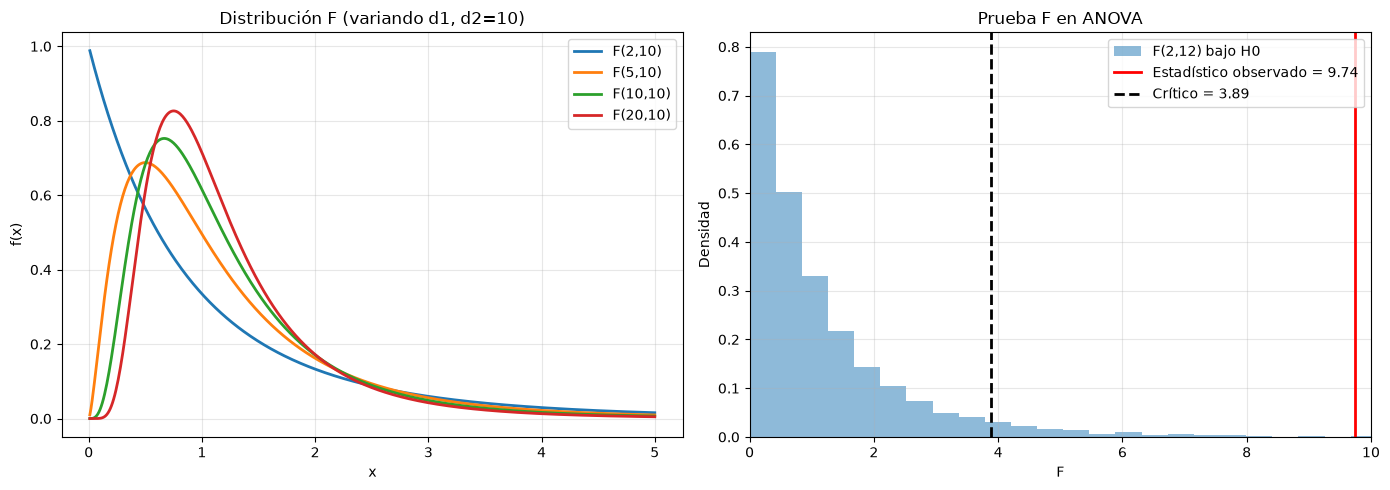
\includegraphics[height=7cm,keepaspectratio=true]{./pe/distF.png}
 % distF.png: 0x0 pixel, 300dpi, 0.00x0.00 cm, bb=
 \caption{Snedecor's $F$-distribution and application to ANOVA.}
 \label{fig:3.2.2}
\end{figure}



\subsection{Sampling Distributions and Data Science}

The sampling distributions studied in this section form the foundation for the most widely used techniques in data science. Below we summarize the main applications.

\subsubsection{Summary Table}

\begin{center}
\begin{tabular}{|l|l|l|}
\hline
\textbf{Distribution} & \textbf{Statistic} & \textbf{Application} \\
\hline
$Z$ (standard normal) & $\dfrac{\bar{X}-\mu}{\sigma/\sqrt{n}}$
& CI for $\mu$ with known $\sigma$; Z-test \\
\hline
Student's $t$ & $\dfrac{\bar{X}-\mu}{S/\sqrt{n}}$
& CI for $\mu$ with unknown $\sigma$; t-test \\
\hline
$\chi^2$ & $\dfrac{(n-1)S^2}{\sigma^2}$
& CI for $\sigma^2$; goodness-of-fit test \\
\hline
Snedecor's $F$ & $\dfrac{S_1^2}{S_2^2}$ or ANOVA
& Comparing variances; ANOVA; F-test in regression \\
\hline
\end{tabular}
\end{center}

\subsubsection{Application 1: A/B Testing}

In A/B testing, two versions of a product are compared by measuring some metric of interest (e.g., conversion rate, time on page).

\begin{ejemplo}
 \label{exmp:3.2.7}
A website has two versions: A (current version) and B (new version). In a test with $n_A = 1000$ users of A, $x_A = 120$ convert. In $n_B = 1000$ users of B, $x_B = 145$ convert. Is there evidence that B is better?
\end{ejemplo}

\begin{solucion}
We estimate the proportions: $\hat{p}_A = 0.120$, $\hat{p}_B = 0.145$. Under the null hypothesis $H_0: p_A = p_B$, the pooled proportion is
\begin{align}
 \hat{p} = \frac{x_A + x_B}{n_A + n_B} = \frac{265}{2000} = 0.1325.
\end{align}
The pooled standard error is
\begin{align}
 \text{SE} = \sqrt{\hat{p}(1-\hat{p})\left(\frac{1}{n_A} + \frac{1}{n_B}\right)}
 = \sqrt{0.1325 \times 0.8675 \times 0.002} \approx 0.01516.
\end{align}
The $Z$-statistic is
\begin{align}
 Z = \frac{\hat{p}_B - \hat{p}_A}{\text{SE}} = \frac{0.145 - 0.120}{0.01516} \approx 1.65.
\end{align}
Under $H_0$, $Z \sim N(0,1)$ approximately. The two-tailed $p$-value is $2(1 - \Phi(1.65)) \approx 0.099$. At the $5\%$ level, we do not reject $H_0$ (though at $10\%$ we would). The result is marginal.
\end{solucion}

\lstinputlisting[language=Python]{../code/distribuciones-muestreo/abTesting.py}

\subsubsection{Application 2: Bootstrap}

The \emph{bootstrap} is a non-parametric technique for estimating the sampling distribution of a statistic through resampling with replacement.

\begin{teorema}[Bootstrap Principle]
Let $X_1, \ldots, X_n$ be an iid sample from an unknown distribution $F$, and $\theta = T(F)$ a parameter of interest. If $\hat{\theta} = T(\hat{F}_n)$ is the plug-in estimator (where $\hat{F}_n$ is the empirical distribution), then the sampling distribution of $\hat{\theta}$ can be approximated by the distribution of $\hat{\theta}^* = T(\hat{F}_n^*)$, where $\hat{F}_n^*$ is obtained by resampling with replacement from the original sample.
\end{teorema}

\begin{ejemplo}
 \label{exmp:3.2.8}
Consider a sample of size $n = 50$ from a population with an unknown distribution. Use the bootstrap to estimate the bias and variance of the sample median.
\end{ejemplo}

\begin{solucion}
\begin{enumerate}
 \item Calculate the observed median $\hat{\theta} = \text{med}(X_1, \ldots, X_{50})$.
 \item For $b = 1, \ldots, B$ (e.g., $B = 10000$):
   \begin{enumerate}
    \item Generate a bootstrap sample $X_1^*, \ldots, X_{50}^*$ by sampling with replacement from the original sample.
    \item Calculate the bootstrap median $\hat{\theta}_b^* = \text{med}(X_1^*, \ldots, X_{50}^*)$.
   \end{enumerate}
 \item Estimate:
   \begin{align}
    \widehat{\text{Bias}}_{\text{boot}} &= \frac{1}{B}\sum_{b=1}^B \hat{\theta}_b^* - \hat{\theta}, \\
    \widehat{\text{Var}}_{\text{boot}}(\hat{\theta}) &= \frac{1}{B-1}\sum_{b=1}^B (\hat{\theta}_b^* - \bar{\hat{\theta}}^*)^2.
   \end{align}
 \item The $95\%$ bootstrap confidence interval is $[\hat{\theta}_{\alpha/2}^*, \hat{\theta}_{1-\alpha/2}^*]$ where the quantiles are taken over $\{\hat{\theta}_b^*\}$.
\end{enumerate}
\end{solucion}

\lstinputlisting[language=Python]{../code/distribuciones-muestreo/bootstrap.py}

\subsubsection{Application 3: Inference in Machine Learning}

In machine learning, sampling distributions underlie:

\begin{itemize}
 \item \textbf{Cross-Validation}: the variance of the generalization error estimator can be estimated using the bootstrap or via the $t$-distribution (with the number of folds determining the degrees of freedom).
 \item \textbf{Hypothesis Testing for Model Comparison}: paired $t$-tests are used to compare two models on the same data, or $F$-tests to compare nested models (e.g., linear regression).
 \item \textbf{Confidence Intervals for Metrics}: precision and recall follow approximately normal distributions for large samples; their CIs are constructed using $Z$ or $t$.
 \item \emph{Feature Selection}: the $F$-test is used to evaluate the global significance of a regression model, and $\chi^2$ tests are used to evaluate independence between categorical variables.
\end{itemize}

\begin{observacion}
In deep learning, classical sampling distributions are less prominent because models are trained on massive volumes of data and evaluated on holdout test sets rather than using classical hypothesis tests. However, they remain fundamental for:
\begin{itemize}
 \item Comparing architectures using hypothesis tests on aggregated performance metrics.
 \item Estimating prediction uncertainty (confidence intervals, conformal prediction).
 \item Quantifying the statistical significance of benchmark improvements.
\end{itemize}
\end{observacion}
